\documentclass[norsk]{beamer}
\usepackage[latin1]{inputenc}

\usepackage{listings}


\lstset{language=Java}

%\usetheme{Warsaw}
\usetheme[sky-200]{UiO}

%\useinnertheme[shadow]{rounded}
\urlstyle{sf}

\title[INF1010]%(optional, only for long titles)
{INF1010 - Felles�velser}
\subtitle{Praktisk gjennomgang av programmeringsteknikker}
\author[Tor Ivar Johansen] % (optional, for multiple authors)
{Tor Ivar Johansen \and Espen Angell Kristiansen}
\institute[Universitetet i Oslo] % (optional)
{
Institutt for informatikk
}
\subject{Objektorientert programmering}

% \AtBeginSection[]
% {
%    \begin{frame}
%        \frametitle{Disposisjon}
%        \tableofcontents[currentsection]
%    \end{frame}
% }



\begin{document}

\begin{frame}
\huge INF1010 - Felles�velse
\end{frame}

 \begin{frame}
 \titlepage 
 \end{frame}

\begin{frame}
\frametitle{Rekursjon}
Gjentakelse/repetisjon i en selvliknende m�te.
\end{frame}

\begin{frame}
  \textbf{Rekursjon} \\
       \hspace{2cm}se rekursjon
\end{frame}

\begin{frame}
  \textbf{Rekursjon} \\
       \hspace{2cm}om du fortsatt ikke forst�r: se rekursjon
\end{frame}

%http://www.post-literate.com/gerpunx/archives/2005/01/prepare_to_lose_your_mind.php

\begin{frame}
  \frametitle{Droste effect}
  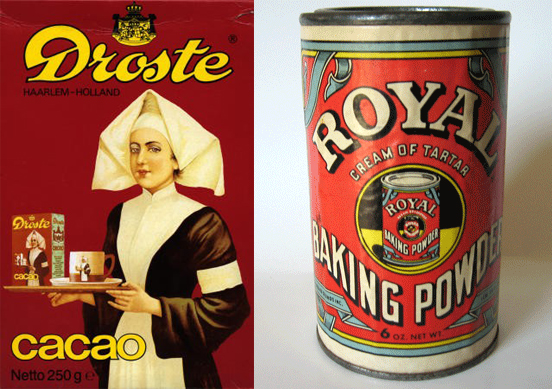
\includegraphics[scale=0.5]{bilder/droste}
\end{frame}

\begin{frame}
  \frametitle{Rekursjon i programmering}
  \begin{itemize}
  \pause \item Divide and conquer
  \pause \item Dele problemer inn i subproblemer av samme type
  \pause \item Basistilfellet bestemmer n�r rekursjonen er over
  \end{itemize}
\end{frame}

%\lstset{language=Java, backgroundcolor=\color{yellow}, basicstyle=8pt, commentstyle=\color{green}}

\begin{frame}[fragile]
  \frametitle{Uendelig rekursjon}
     \begin{lstlisting}
       void forever() {
         forever();
       }
     \end{lstlisting}

\end{frame}



\end{document}
